\section{GoCD}
    Systém GoCD vychází z~projektu Cruise~\cite{thoughtworks-gocd}. Oba projekty vznikly ve firmě ThoughtWorks, kde pracoval průkopník a zastánce praktik \textit{extrémního programování} M. Fowler~\cite{fowler-go}. Fowler systém Cruise doporučoval ve známém článku o~\CI~\cite{fowler-ci}.

    \subsection{Architektura GoCD, možnosti konfigurace}
        GoCD stejně jako většina ostatních \CI staví na architektuře jednoho kontrolního serveru a řadě interních nebo externích agentů, které se starají o~spuštění jednotlivých jobů. Ve výchozím nastavení jsou data persistována v~embedované H2 databázi na server procesu. Instalace GoCD je díky tomu jednoduchá, protože stačí zaregistrovat externí repozitář a nainstalovat balíček pro server a pro agenty.

        Po prvním zobrazení webového rozhraní serveru se zobrazuje quick-start, který provádí vytvořením nové pipeline. Přestože GoCD podporuje \textit{Pipelines as code}, očekávaný primární vstup je klikání v~administraci~\cite{gocd-pas}. Načítání externích souborů je vyřešeno rozšířením, jehož použití se definuje v~hlavní \glstext{XML} konfiguraci na webu. Separovaná konfigurace tak není kompletní a závisí na další ruční konfiguraci.

    \subsection{Rozšiřitelnost}
        GoCD nabízí několik možností, jak rozšiřovat výchozí funkcionalitu pomocí pluginů~\cite{gocd-extensions}. Na rozdíl od Jenkins, kde lze upravit prakticky cokoliv, vystavuje pro pluginy GoCD jenom některá \glstext{API}. Nelze tak například ovlivňovat uživatelské rozhraní.

        Zhruba 80 pluginů je na oficiálním registru~\cite{gocd-plugins}. ThoughtWorks~Inc.~zaštiťují 8 pluginů a a z~toho je 6 placených.

        Z~veřejně dostupných rozšíření jsou všechna kromě jednoho hostována na GitHub. Jak jsem ale vizualizoval \pfxref{v~grafu}{fig:jenkins-plugins}, GoCD rozšíření jsou ještě hůř udržovaná než ta pro Jenkins. A~to je jich méně než dvacetina.

        \begin{iffigure}
            \centering
            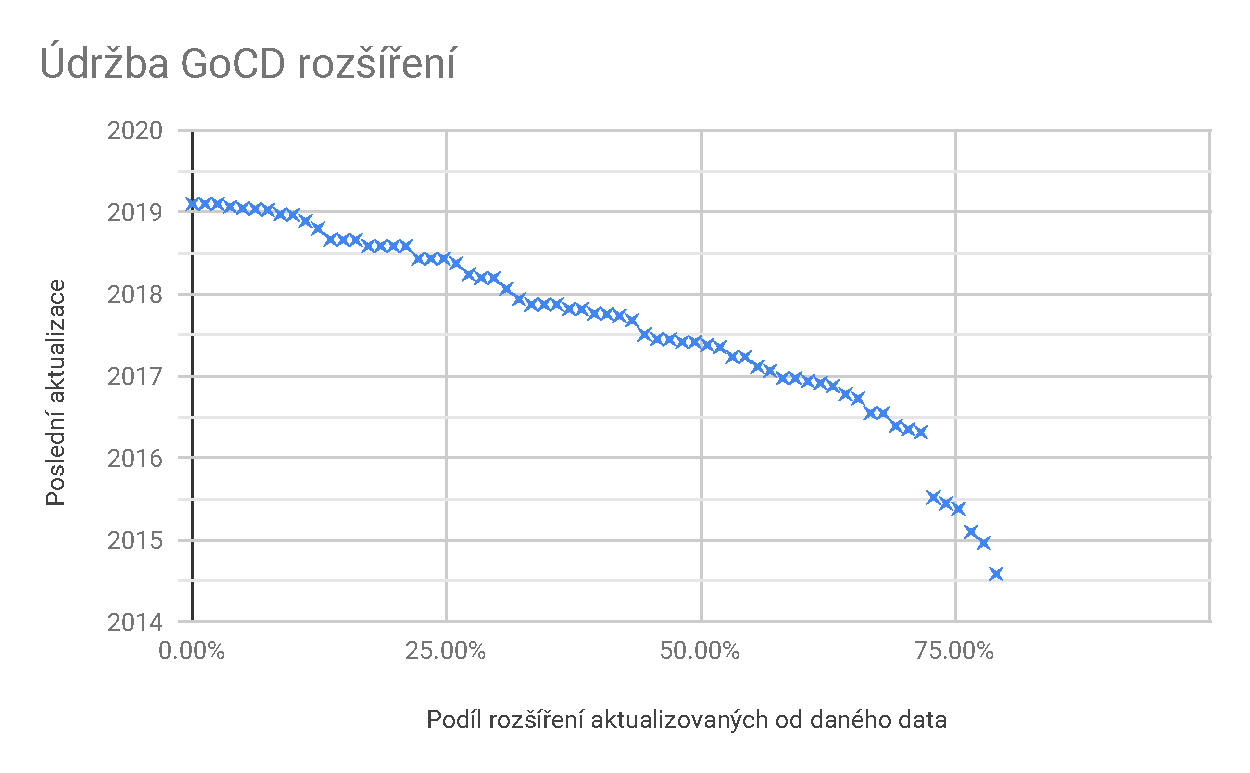
\includegraphics[width=\textwidth,height=9cm,keepaspectratio]{media/go-plugins-update.pdf}
            \caption{Rozdělení podle poslední aktualizace. Pouze 17 rozšíření (20 \%) bylo aktualizováno v~posledním půl roce. Pouhých 30~\% rozšíření mělo alespoň jednu aktualizaci za poslední rok. Přibližně 20 \% rozšíření nemá žádné stabilní vydání. Zdroj: data vytěžena z~GitHub repozitářů, dostupná na přiloženém mediu v~\code{appendix/gocd-plugins.csv}.}
            \label{fig:jenkins-plugins}
        \end{iffigure}

    \newpage
    \subsection{Zabezpečení}
        Po instalaci serveru je v~základu celá administrace dostupná pro všechny, bez autorizace. Lze zapnout zabudovaná rozšíření, která zprovozní přihlášení heslem a nebo přes \glstext{LDAP}. Nic v~\glstext{UI} k~tomu ale správce nenabádá. Velmi překvapivě ale není v~Shodan databázi žádná nezabezpečená instance GoCD na výchozím portu~\cite{shodan-gocd}.

        Izolace klientů závisí na použitých agentech. Klasický agent používá sdílené prostředí a zdroje, ale GoCD podporuje tzv.~\textit{Elastic Agent}, které se zapínají a vypínají dynamicky podle poptávky. Lze je využít pro zapnutí nového prostředí v~Dockeru, Kubernetes, OpenStacku a několika dalších. Tato jednorázová prostředí nabízí lepší izolaci. Nenašel jsem rozšíření, které by dokázalo spravovat Elastic Agents pro VMware nebo jiný virtualizační nástroj, který by měl ještě lepší izolaci klientů.

        Na webu \glstext{CVE} Details jsem pro GoCD nenašel žádná historická \glstext{CVE}. Projekt ale využívá platformu HackerOne, kde za poslední tři roky zpracovali 39 nahlášených chyb~\cite{gocd-hackerone}. Ze zveřejněných reportů je vidět, že správci reagují rychle a bezpečnostní chyby opravují v~co nejkratším možném termínu.

    \subsection{Dostupnost}
        GoCD agenti jsou z~principu stavové aplikace a stejně jako u~všech ostatních \CI jejich výpadek způsobí, že přijdeme o~spuštěné joby. Může jich ale běžet mnoho a pomocí rolling update je lze aktualizovat bez výpadku.

        Server je bohužel také stavový a může běžet pouze v~jedné replice. GoCD prodává velmi drahý \textit{Business Continuity Addon}, který dokáže udržovat standby repliku~\cite{gocd-ha}. Failover proces ale není nijak automatizovaný a povýšení na primární repliku vyžaduje restart GoCD serveru. U~GoCD nelze udělat perfektní HA bez ztráty žádného požadavku když vypadne primární replika.

        Upgrade serveru na novější verzi vyžaduje restart a tím pádem nedostupnost celého prostředí. Navíc se při startu nové verze aplikace automaticky spustí databázové migrace, které na větších instancích podle dokumentace mohou trvat přes 10 minut~\cite{gocd-upgrading}. Celkově je tak při rutinní aktualizaci potřeba počítat s~výpadkem minimálně 15 minut.

        GoCD má jednoduchý proces pro vytvoření zálohy, který lze spustit buď z~\glstext{UI} nebo z~\glstext{API}~\cite{gocd-backup}. Záloha obsahuje dump databáze, vyklikané \glstext{XML} konfigurace aplikace a konfigurace repozitářů, nastavení webového serveru a klíče. Nejsou zálohovány historie a výstupy spuštěných úloh, ani nainstalovaná rozšíření! Proces vytváří archiv na disku aktuálního serveru, který je poté dobré zmigrovat na nějaké externí úložiště.

    \subsection{Integrace}
        Lze propojit GoCD s~dalšími nástroji; některé funkce -- především ty co mají vliv na \glstext{UI} -- jsou vestavěné. To je například odkazování na externí správu úkolů podle regulárního výrazu. Ostatní integrace jsou dostupná jako rozšíření, která je nutné doinstalovat: mezi ně patří například oznámení stavu na GitHub/Stash/Gerrit a podobně. Pro Bitbucket ani Gitlab podpora neexistuje. Lze ji ale doprogramovat jako nové rozšíření.

    \begin{figure}[H]
        \centering
        \begin{minted}[frame=lines,framesep=2mm,linenos]{xml}
<?xml version="1.0" encoding="utf-8"?>
<pipeline name="p2">
  <materials>
    <git url="file:///src/p2-dynamic/" shallowClone="true" />
  </materials>
  <stage name="BuildStage">
    <jobs>
      <job name="BuildJob">
        <tasks>
          <exec command="make">
            <arg>build</arg>
            <runif status="passed" />
          </exec>
          <exec command="make">
            <arg>deploy</arg>
            <runif status="passed" />
          </exec>
        </tasks>
      </job>
    </jobs>
  </stage>
</pipeline>
        \end{minted}
        \caption{Přestože GoCD je primárně určeno ke konfiguraci z \glstext{GUI}, lze editovat přímo konfigurační \glstext{XML} soubory. Vzhledem k chybějící izolaci úkonů v tomto \CI byla tato pipeline navržena jako prosté spuštění dvou příkazů.}
    \end{figure}


        Navzdory svému jménu nenabízí GoCD žádnou podporu pro continuous deployment. Ve webovém rozhraní (ani jinde) není možnost spravovat nasazená prostředí a verze aplikací, podpora pro ručně potvrzené kroky je velmi limitovaná, a integrace s~Kubernetes/OpenShift nebo jiným  nebo neexistuje.

    \subsection{Praktické nasazení projektů}
        \subsubsection{Projekt 1}
            Nasazení GoCD pro statický projekt bylo vesměs stejné, jako u~GitLab shell executoru: na server jsem předinstalovat Ruby a v~rámci pipeline se pak pouze volá instalace Ruby gems a samotná kompilace. Narazil jsem na drobný problém při použití \glstext{RVM} (správce Ruby verzí), který dynamicky upravuje \code{\$PATH}, ale GoCD tato nastavení nerespektoval. Musel jsem tak ručně cestu k~Ruby upravit v~souboru \code{.profile} a restartovat GoCD agent aby se změny projevily.

        \subsubsection{Projekt 2}
            Pro druhý ukázkový projekt byla implementace v~GoCD velmi jednoduchá, protože jsem závislosti předinstaloval při tvorbě prostředí. Pro víc projektů je to nepraktické řešení, ale pokud bude v~systému vždy pouze jeden projekt využívající dané knihovny a podpůrný software, nenarazíme na skoro žádné problémy. Obtížnější az neřešitelné může být testování zároveň několika verzí závislostí (například současná stabilní verze a nejnovější nestabilní verze).

        \subsubsection{Projekt 3}
            Při implementaci \CI pro kontejnerizovaný projekt jsem narazil na to, že GoCD neinterpoluje proměnné prostředí. Je tak nutné explicitně volat \code{sh -c "\$CMD"}, což je zbytečná komplikace bez jasných výhod. Dále jsem se potýkal s~tím, že GoCD nedefinuje běžné proměnné prostředí. Konkrétně \code{CI\_COMMIT\_SHA} je dostupné jen pod názvem \code{GO\_REVISION}. Přes tyto nedostatky poskytuje GoCD možnosti pro kompilaci a nasazení kontejnerizované aplikace.
